\subsubsection{DimeNet and DimeNet++}
\label{subsubsec:dimenet}

DimeNet (\enquote{Directional Message Passing Neural Network}) 
\cite{DBLP:journals/corr/abs-2003-03123}, which was proposed by Gasteiger et al. 
in 2020, is an energy-centric GNN architecture for predicting energies and forces 
of molecule structures. DimeNet does not only consider pairwise distances between atoms, 
but also takes advantage of directional information. In the EGN 
language (see \ref{subsubsec:egns} and \cite{https://doi.org/10.48550/arxiv.2203.09697}),
3-way interactions between nodes are modeled.

Just as in \eqref{eq:molecule_setup}, the network receives the positions $\XX$
and atomic numbers $\zz$ of a molecule as inputs. 
At first, define the pairwise distances and relative direction vectors
\[
    d_{ij} \: \coloneqq \: \norm{\xx_j - \xx_i}_2, 
    \qquad \vec{\xx}_{ij} \: \coloneqq \xx_j - \xx_i \text{.}
\]
In the beginning, a molecular graph is given or it is defined by connecting the atoms with distance 
below some threshold $c$. Denote by $\mathcal{N}_i \subseteq \set{1, \dots, n}$ the 
neighborhood of the atom $i$.
Directional information is now leveraged by also 
taking the angles
\[
    \alpha_{kji} \: \coloneqq \: \measuredangle\left( \vec{\xx}_{jk}, \vec{\xx}_{ji} \right)
\]
between neighboring edges $(\_,k,j)$ and $(\_,j,i)$ into account. 
The distances and angles are then transformed to a representation which is related
to DFT calculations \cite[Section 5]{DBLP:journals/corr/abs-2003-03123}
by using radial and spherical Bessel functions:
\[
    \ee_{\text{RBF}}^{(ji)} \: \coloneqq \: \ee_{\text{RBF}}(d_{ji}), 
    \qquad \aaa_{\text{SBF}}^{(kji)} \: \coloneqq \: \aaa_{\text{SBF}}(d_{kj}, \alpha_{kji})
    \text{.}
\]
In an embedding phase, edge embeddings $\mm_{ji}^{(1)}$ and outputs
$t_{i}^{(1)}$ or a global attribute $t^{(1)} = \sum_{i=1}^n t_i^{(1)}$ are initialized based
on the atomic numbers $\zz$ and $\ee_{\text{RBF}}^{(ji)}$. Both node embedings 
$\hh_i \coloneqq \sum_{j \in \mathcal{N}_i} \mm_{ji}$ and triplet embeddings are handled
implicitly (i.e. the \textbf{Triplet Update} and \textbf{Node Update} outputs from 
\ref{subsubsec:gns}, \ref{subsubsec:egns} do not depend on their respective predecessors).
From now on, we denote implicit or irrelevant embeddings by \enquote{$\_$}.

In the EGN language, the initial graph is defined as follows:
\[
    G \: = \: (t^{(1)}, V^{(1)}, E^{(1)}, T^{(1)})
\]
with nodes, edges and triplets
\begin{align*}
    V^{(1)} \: &\coloneqq \: \setcomp{\hh_i^{(1)}}{i \in \set{1, \dots, n}}, \\
    E^{(1)} \: &\coloneqq \: \setcomp{(\mm_{ji}^{(1)}, i, j)}
    {i, j \in \set{1, \dots, n}, d_{ji} \leq c}, \\
    T^{(1)} \: &\coloneqq \: \setcomp{(\_,(\mm_{kj}^{(1)}, j, k), (\mm_{ji}^{(1)}, i, j))}
    {i, j, k \in \set{1, \dots, n}, \; d_{ji}, d_{kj} \leq c} \text{;}
\end{align*}
i.e. the triplets are all possible paths of length two on the edges of $G$.

After this initial graph embedding has been computed, a series of EGN blocks,
here called \textit{interaction blocks}, are applied to the graph.

Within such an interaction block, the edge embeddings 
are updated as follows (i.e. corresponds to \textbf{Edge Update}):
\[
    \mm_{ji}^{(l+1)} \: = \: 
    f_{\text{update}}\Bigg(\mm_{ji}^{(l)}, 
    \underbrace{\sum_{k \in \mathcal{N}_{j} \backslash\{i\}}}_{\textbf{Triplet Aggr.}} 
    \underbrace{ \vphantom{\sum_{\mathcal{N}_j}} 
    f_{\text {int }}\left(\mm_{k j}^{(l)}, \ee_{\text{RBF}}^{(ji)}, 
    \aaa_{\text{SBF}}^{(kj, ji)}\right)}
    _{\textbf{Triplet Update}}\Bigg) \text{,}
\]
where $f_{\text{int}}$ and $f_{\text{update}}$ are implemented by neural networks.
These edge embeddings are then directly aggregated to the new node embeddings
\[
    \hh_i^{(l+1)} \: = \: \sum_{j \in \mathcal{N}_i} \mm_{ji}^{(l+1)}
\]
and the outputs $t^{(l+1)}_i$ as well as the global attribute $t^{(l+1)}$ are
updated (based on another \textbf{Edge Aggregation} step).
Finally, the global output $t$ that represents the molecule's energy is 
aggregated over all interaction block outputs.
The whole DimeNet architecture as depicted in its original paper 
\cite{DBLP:journals/corr/abs-2003-03123} can be seen in Figure~\ref{fig:dimenet}.

DimeNet++ \cite{https://doi.org/10.48550/arxiv.2011.14115} is an upgraded version of 
DimeNet that increases the efficiency of training without impacting the quality of results. 
These improvements include replacing the bilinear layer in the directional message passing 
step by a simpler Hadamard product, downprojecting the embeddings into lower dimensions in
computation-intensive parts of the model and up-project them back to the original dimensions 
after these layers, and using less interaction layers.

\begin{figure}[H]
    \centering
    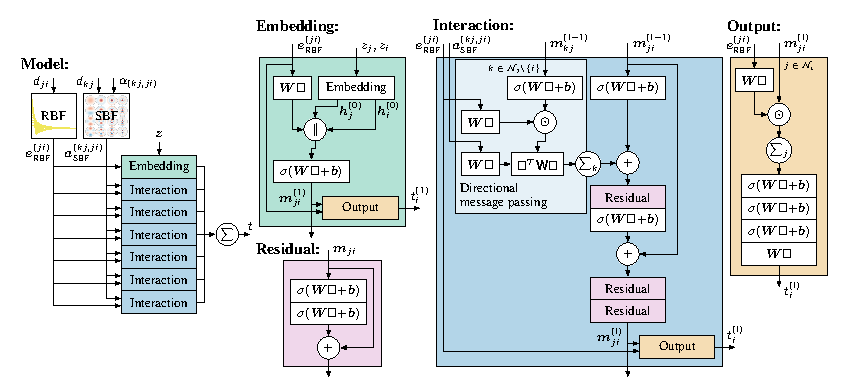
\includegraphics[]{atomic_simulations/dimenet.pdf}
    \caption{The original DimeNet architecture as depicted in \cite*{DBLP:journals/corr/abs-2003-03123}.}
    \label{fig:dimenet}
\end{figure}
